\documentclass[12pt, titlepage]{article}

\usepackage{graphicx}
\usepackage{float}
\usepackage{booktabs}
\usepackage{longtable}
\usepackage{tabularx}
\usepackage{hyperref}
\hypersetup{
    colorlinks,
    citecolor=black,
    filecolor=black,
    linkcolor=red,
    urlcolor=blue
}
\usepackage[round]{natbib}

%% Comments

\usepackage{color}

\newif\ifcomments\commentstrue %displays comments
%\newif\ifcomments\commentsfalse %so that comments do not display

\ifcomments
\newcommand{\authornote}[3]{\textcolor{#1}{[#3 ---#2]}}
\newcommand{\todo}[1]{\textcolor{red}{[TODO: #1]}}
\else
\newcommand{\authornote}[3]{}
\newcommand{\todo}[1]{}
\fi

\newcommand{\wss}[1]{\authornote{blue}{SS}{#1}} 
\newcommand{\plt}[1]{\authornote{magenta}{TPLT}{#1}} %For explanation of the template
\newcommand{\an}[1]{\authornote{cyan}{Author}{#1}}

%% Common Parts

\newcommand{\progname}{Software Engineering} % PUT YOUR PROGRAM NAME HERE
\newcommand{\authname}{Team \#11, OKKM Insights
\\ Mathew Petronilho
\\ Oleg Glotov
\\ Kyle McMaster
\\ Kartik Chaudhari} % AUTHOR NAMES                  

\usepackage{hyperref}
    \hypersetup{colorlinks=true, linkcolor=blue, citecolor=blue, filecolor=blue,
                urlcolor=blue, unicode=false}
    \urlstyle{same}
                                


\begin{document}

\title{Verification and Validation Report: \progname} 
\author{\authname}
\date{\today}
	
\maketitle

\pagenumbering{roman}

\section{Revision History}

\begin{tabularx}{\textwidth}{p{3cm}p{2cm}X}
\toprule {\bf Date} & {\bf Version} & {\bf Notes}\\
\midrule
Date 1 & 1.0 & Notes\\
Date 2 & 1.1 & Notes\\
\bottomrule
\end{tabularx}

~\newpage

\section{Symbols, Abbreviations and Acronyms}

\renewcommand{\arraystretch}{1.2}
\begin{tabular}{l l} 
  \toprule		
  \textbf{symbol} & \textbf{description}\\
  \midrule 
  T & Test\\
  \bottomrule
\end{tabular}\\

\wss{symbols, abbreviations or acronyms -- you can reference the SRS tables if needed}

\newpage

\tableofcontents

\listoftables %if appropriate

\listoffigures %if appropriate

\newpage

\pagenumbering{arabic}

This document ...

\section{Functional Requirements Evaluation}
\subsection{Summary of Tests}
\begin{tabular}{|c|c|l|}
    \hline
    \textbf{Test ID} & \textbf{Status} & \textbf{Notes}\\
    \hline
    T-FR0 & Pass & \\
    T-FR1 & Pass & \\
    T-FR2 & Pass & Not all fields from test are in user information\\
    T-FR3 & N/A & Requirement covered is out of scope\\
    T-FR4 & Pass & Confirmed Payment no longer required\\
    T-FR5 & Pass & Download not yet supported\\
    T-FR6 & Fail & Large image files fail to upload\\
    T-FR7 & Fail & Not yet implemented \\ 
    T-FR8 & Fail & Not yet implemented \\ 
    T-FR9 & Pass & \\
    T-FR10 & Pass & \\
    T-FR11 & Pass & \\
    T-FR12 & N/A & Requirement covered is out of scope\\
    T-FR13 & Pass & \\
    T-FR14 & Fail & Not yet implemented \\\hline
\end{tabular}


\subsubsection*{T-FR0: Customer Account Creation}

\begin{enumerate}
    \item \textbf{Initial State}: The system is accessible, and no user account currently exists for the test user.
    \item \textbf{Input}:
    \begin{itemize}
        \item Customer provides valid personal information:
        \begin{itemize}
            \item \textbf{Name}: ``Alice Smith''
            \item \textbf{Email}: \texttt{alice.smith@example.com}
            \item \textbf{Password}: ``StrongPassword!2021''
        \end{itemize}
        \item Customer agrees to the system's privacy policy.
    \end{itemize}
        \item \textbf{Expected Result}:
        \begin{itemize}
            \item A new user account is created.
            \item Account information is securely stored in the database.
            \item The customer is redirected to the login page with a success message.
        \end{itemize}
        \item \textbf{Result}: Pass
\end{enumerate}
\subsubsection*{T-FR1: Customer Authentication}

\begin{enumerate}
    \item \textbf{Initial State}: An existing user account with the following credentials:
    \begin{itemize}
        \item \textbf{Email}: \texttt{user.test@example.com}
        \item \textbf{Password}: ``TestPass\#123''
    \end{itemize}
    \item \textbf{Input}:
    \begin{itemize}
        \item Customer enters the correct login credentials:
        \begin{itemize}
            \item \textbf{Email}: \texttt{user.test@example.com}
            \item \textbf{Password}: ``TestPass\#123''
        \end{itemize}
    \end{itemize}

        \item \textbf{Expected Result}:
        \begin{itemize}
            \item Customer is successfully authenticated.
            \item Access to privileged information (e.g., user dashboard) is granted.
            \item A session token or cookie is established for the user session.
        \end{itemize}
        \item \textbf{Result}: Pass
\end{enumerate}

\subsubsection*{T-FR2: Customer Account Modification}

\begin{enumerate}
    \item \textbf{Initial State}: Customer is logged in and has access to their account information page.
    \item \textbf{Input}:
    \begin{itemize}
        \item Customer updates personal information fields:
        \begin{itemize}
            \item \textbf{Address}: ``123 New Street, Cityville''
            \item \textbf{Phone Number}: ``555-1234''
            \item \textbf{Profile Picture}: Uploads a new image file.
        \end{itemize}
    \end{itemize}
    
        \item \textbf{Expected Result}:
        \begin{itemize}
            \item Updated personal information is saved and reflected in the database.
            \item The user receives a confirmation message indicating successful update.
        \end{itemize}
        \item \textbf{Result}: Pass
        \item \textbf{Comments}: Not all fields are used in customer profile. However, functionality remains testable and validated.
\end{enumerate}

\subsubsection*{T-FR3: Payment Processing}

\begin{enumerate}
    \item \textbf{Initial State}: Customer is logged in and ready to make a payment for a service request.
    \item \textbf{Input}:
    \begin{itemize}
        \item Valid payment information:
        \begin{itemize}
            \item \textbf{Credit Card Number}: ``4111 1111 1111 1111'' (Test Visa number)
            \item \textbf{Expiry Date}: ``12/25''
            \item \textbf{CVV}: ``123''
            \item \textbf{Billing Address}: Matches the address on file.
        \end{itemize}
    \end{itemize}
        \item \textbf{Expected Result}:
        \begin{itemize}
            \item Payment is processed successfully.
            \item A confirmation receipt is generated and emailed to the customer.
            \item The service request status is updated to ``Paid'' or equivalent.
        \end{itemize}
        \item \textbf{Result}: Test not completed
        \item \textbf{Comments}: Requirement is out of scope
\end{enumerate}

\subsubsection*{T-FR4: Service Request Submission}

\begin{enumerate}

    \item \textbf{Initial State}: Customer is logged in and has a confirmed payment.
    \item \textbf{Input}:
    \begin{itemize}
        \item Customer fills out the service request form with necessary details:
        \begin{itemize}
            \item \textbf{Service Type}: ``Image Analysis''
            \item \textbf{Description}: ``Analysis of satellite images for deforestation.''
            \item \textbf{Preferred Completion Date}: ``2023-12-31''
        \end{itemize}
    \end{itemize}

        \item \textbf{Expected Result}:
        \begin{itemize}
            \item Service request is accepted and logged in the system.
            \item Customer receives a confirmation message and request ID.
        \end{itemize}
        \item \textbf{Result}: Pass
        \item \textbf{Comments}: Payment is no longer required in initial state.
\end{enumerate}

\subsubsection*{T-FR5: Service Report Delivery}

\begin{enumerate}
    
    \item \textbf{Initial State}: Customer is logged in and has a completed service request.
    \item \textbf{Input}:
    \begin{itemize}
        \item Customer navigates to the ``My Reports'' section after being notified of service completion.
    \end{itemize}
    
        \item \textbf{Expected Result}:
        \begin{itemize}
            \item The service report is available for viewing and download.
            \item Report contents are accurate and correspond to the service request.
        \end{itemize}
        \item \textbf{Result}: Pass
        \item \textbf{Comments}: Download not yet supported
\end{enumerate}

\subsubsection*{T-FR6: Image Upload}

\begin{enumerate}
    \item \textbf{Initial State}: Customer is logged in with an active service request requiring image uploads.
    \item \textbf{Input}:
    \begin{itemize}
        \item Customer uploads multiple image files:
        \begin{itemize}
            \item \texttt{Image1.jpg}: 2\,MB
            \item \texttt{Image2.png}: 3\,MB
            \item \texttt{Image3.tif}: 5\,MB
        \end{itemize}
    \end{itemize}
        \item \textbf{Expected Result}:
        \begin{itemize}
            \item All images are successfully uploaded and stored.
            \item Images are correctly linked to the specific service request.
            \item Customer receives an upload success message.
        \end{itemize}
        \item \textbf{Result}: Fail
        \item \textbf{Comments}: Large image files do not upload
\end{enumerate}

\subsubsection*{T-FR7: Satellite Image Request}

\begin{enumerate}
    \item \textbf{Initial State}: Customer is logged in with an active service request that requires satellite images.
    \item \textbf{Input}:
    \begin{itemize}
        \item Geographic coordinates:
        \begin{itemize}
            \item \textbf{Latitude}: $37.7749^\circ$ N
            \item \textbf{Longitude}: $122.4194^\circ$ W (San Francisco, CA)
            \item \textbf{Date Range}: ``2023-01-01'' to ``2023-01-31''
        \end{itemize}
    \end{itemize}
        \item \textbf{Expected Result}:
        \begin{itemize}
            \item The system retrieves and stores satellite images corresponding to the provided coordinates and date range.
            \item Customer is notified of successful retrieval.
        \end{itemize}
        \item \textbf{Result}: Fail
        \item \textbf{Comments}: Not yet implemented
\end{enumerate}

\subsubsection*{T-FR8: Service Request Failure Alert}

\begin{enumerate}

    \item \textbf{Initial State}: Customer has initiated a service request that cannot be fulfilled due to invalid parameters.
    \item \textbf{Input}:
    \begin{itemize}
        \item Service request with unfulfillable criteria:
        \begin{itemize}
            \item \textbf{Service Type}: ``Image Analysis''
            \item \textbf{Geographic Coordinates}: Invalid coordinates (e.g., Latitude: $95^\circ$ N)
        \end{itemize}
    \end{itemize}
    
        \item \textbf{Expected Result}:
        \begin{itemize}
            \item Customer receives an alert indicating that the service request cannot be processed.
            \item An explanation of the failure is provided.
        \end{itemize}
        \item \textbf{Result}: Fail
        \item \textbf{Comments}: Not yet implemented
\end{enumerate}

\subsubsection*{T-FR9: Labeler Account Creation}

\begin{enumerate}
    \item \textbf{Initial State}: No labeler account exists for the test user in the system.
    \item \textbf{Input}:
    \begin{itemize}
        \item Labeler provides required account information:
        \begin{itemize}
            \item \textbf{Name}: ``Bob Labeler''
            \item \textbf{Email}: \texttt{bob.labeler@example.com}
            \item \textbf{Password}: ``LabelerPass789!''
            \item \textbf{Expertise Area}: ``Satellite Image Annotation''
        \end{itemize}
    \end{itemize}
        \item \textbf{Expected Result}:
        \begin{itemize}
            \item A new labeler account is created and securely stored.
            \item Labeler is prompted to complete any additional on-boarding steps.
        \end{itemize}
        \item \textbf{Result}: Pass
\end{enumerate}

\subsubsection*{T-FR10: Labeler Authentication}

\begin{enumerate}
    \item \textbf{Initial State}: Labeler account exists with credentials:
    \begin{itemize}
        \item \textbf{Email}: \texttt{labeler.test@example.com}
        \item \textbf{Password}: ``LabelerSecure!2022''
    \end{itemize}
    \item \textbf{Input}:
    \begin{itemize}
        \item Labeler enters correct login credentials.
    \end{itemize}
        \item \textbf{Expected Result}:
        \begin{itemize}
            \item Labeler is authenticated successfully.
            \item Access to the labeler dashboard is granted.
        \end{itemize}
        \item \textbf{Result}: Pass
\end{enumerate}

\subsubsection*{T-FR11: Labeler Account Modification}

\begin{enumerate}
    \item \textbf{Initial State}: Labeler is logged in and on the account settings page.
    \item \textbf{Input}:
    \begin{itemize}
        \item Update personal information:
        \begin{itemize}
            \item \textbf{Expertise Area}: Add ``Aerial Photography Annotation''
            \item \textbf{Contact Number}: ``555-6789''
        \end{itemize}
    \end{itemize}
        \item \textbf{Expected Result}:
        \begin{itemize}
            \item Personal information is updated and stored in the database.
            \item Labeler receives a confirmation of successful update.
        \end{itemize}
        \item \textbf{Result}: Pass
\end{enumerate}

\section*{FR12: Labeler Earnings Transfer Test}

\begin{enumerate}
    \item \textbf{Initial State}: Labeler is logged in with available earnings exceeding the minimum transfer threshold.
    \item \textbf{Input}:
    \begin{itemize}
        \item Transfer request to linked banking platform:
        \begin{itemize}
            \item \textbf{Amount}: Total available earnings.
            \item \textbf{Bank Account Details}: Pre-verified and linked.
        \end{itemize}
    \end{itemize}
        \item \textbf{Expected Result}:
        \begin{itemize}
            \item Earnings are transferred successfully.
            \item Transaction record is created.
            \item Labeler receives confirmation and updated earnings balance.
        \end{itemize}
        \item \textbf{Result}: Test not completed
        \item \textbf{Comments}: Requirement is out of scope
\end{enumerate}

\subsubsection*{T-FR13: Image Annotation}

\begin{enumerate}
    \item \textbf{Initial State}: Labeler is logged in with images assigned for annotation.
    \item \textbf{Input}:
    \begin{itemize}
        \item Labeler annotates an image using the provided tools:
        \begin{itemize}
            \item Draws bounding boxes around objects.
            \item Adds classification labels to each object.
            \item Saves the annotation.
        \end{itemize}
    \end{itemize}

        \item \textbf{Expected Result}:
        \begin{itemize}
            \item Annotated image is stored in the system.
            \item Annotation data is correctly linked to the image and service request.
            \item Labeler receives confirmation of successful submission.
        \end{itemize}
        \item \textbf{Result}: Pass
\end{enumerate}

\subsubsection*{T-FR14: Consolidated Annotation Report}

\begin{enumerate}
    \item \textbf{Initial State}: All required labeler annotations are complete for a service request.
    \item \textbf{Input}:
    \begin{itemize}
        \item System triggers consolidation process for annotations.
    \end{itemize}
        \item \textbf{Expected Result}:
        \begin{itemize}
            \item Consolidated report is generated if label accuracy meets the predefined threshold.
            \item Report is stored and made accessible to the customer.
        \end{itemize}
        \item \textbf{Result}: Fail
        \item \textbf{Comments}: Not yet implemented.
\end{enumerate}

\subsection{Analysis}

Overall, the validation team is happy with the progress towards satisfying our refined functional requirements. Of the 13 attempted tests, nine were successful. Of the four which were unsuccessful,
only one failed due to some error related to implementation. The others are expected to fail, as they have yet to be implemented. The unexpected failure is `T-FR6', which has showed that large image files are unable to be uploaded to the 
project creation portal. The team has been able to trace this error back to our web hosting platform, and are in the process of identifying potential fixes. After this fix, and the implementation of report creation and satellite image requests, we will have demonstrated 100\% functional requirement validation.

\section{Nonfunctional Requirements Evaluation}
\subsection{Look and Feel}
\subsubsection{Summary of Tests}
\begin{center}
    \begin{tabular}{|c|c|l|}
        \hline
        \textbf{Test ID} & \textbf{Status} & \textbf{Notes}\\
        \hline
        T-LF0 & Pass & \\
        T-LF1 & Pass & \\
        T-LF2 & Pass & \\
        \hline
    \end{tabular}
\end{center}
    
\begin{enumerate}
    \item{T-LF0: Responsive Layout Validation\\}
        
    \textbf{Initial State}: Users access the application on devices with screen resolutions ranging from 1024$\times$768 pixels to 1920$\times$1080 pixels.
    
    \textbf{Input/Condition}: The application is displayed on various screen sizes within the specified range to verify adaptability and layout consistency.

    \textbf{Expected Result}: All elements are displayed on the screen, regardless of dimensions.

    \textbf{Result} Pass

    \item{T-LF1: Interactive Elements Feedback Validation\\}
    
    \textbf{Initial State}: Interactive elements (e.g., buttons, links) are present within the application interface.
    
    \textbf{Input/Condition}: Users interact with various interactive elements to verify that visual feedback is provided appropriately.
    
    \textbf{Expected Result}: Each interactive element provides feedback when hovered over and clicked on.

    \textbf{Result} Pass
    
    \item{T-LF2: Unified Visual Design Validation\\}
    
    
    \textbf{Initial State}: The application interface displays all components (buttons, menus, text fields, images, etc.) with the unified visual design specifications.
    
    \textbf{Input/Condition}: Users or testers navigate through the application to assess the consistency of font type, sizing, color, and background tones across all components.
    
    \textbf{Expected Result}: All elements follow consistent style

    \textbf{Result} Pass

    \textbf{Comments} Replacing Label Studio with our own framework was necessary to pass this test.
    
    \end{enumerate}

    \subsubsection{Analysis}
    All three of the Look and Feel tests pass. These tests were designed to provide complete coverage of the Look and Feel requirements, and therefore we believe them to be covered.
\subsection{Usability}
	Please see usability report, found \href{https://github.com/OKKM-insights/OKKM.insights/blob/main/docs/Extras/UsabilityReport/UsabilityReport.pdf}{here}

\subsection{Performance}
\begin{longtable}{|c|c|l|}
    \hline
    \textbf{Test ID} & \textbf{Status} & \textbf{Notes} \\
    \hline
    T-PR0 & Pass & \textit{New User Account Processing Time Validation} \\
    T-PR1 & Pass & \textit{Service Request Completion Time Validation} \\
    T-PR2 & Pass & \textit{Next Image Serving Time Validation} \\
    T-PR3 & Removed & \textit{Payout Processing Time Validation (Out of Scope)} \\
    \hline
\end{longtable}

\subsubsection{T-PR0: New User Account Processing Time Validation}
\textbf{Initial State}: The system is ready to accept new user account creation requests.\\
\textbf{Input/Condition}: A set of new user account creation requests are submitted, and their processing times are tracked.\\
\textbf{Expected Result}: At least MIN ACCOUNT CREATION SUCCESS\% of requests are processed within 15 minutes, and all within 48 hours.\\
\textbf{Result}: \textbf{Pass}

\subsubsection{T-PR1: Service Request Completion Time Validation}
\textbf{Initial State}: The system is ready to accept service requests with predefined negotiated time limits.\\
\textbf{Input/Condition}: Service requests are submitted under typical operating conditions.\\
\textbf{Expected Result}: At least MIN REPORT RETURN\% of requests are completed within the negotiated time limit, and all within an additional 48-hour buffer.\\
\textbf{Result}: \textbf{Pass}

\subsubsection{T-PR2: Next Image Serving Time Validation}
\textbf{Initial State}: Labelers are logged in with images available for labeling.\\
\textbf{Input/Condition}: Labelers request the next image while images are available in the queue.\\
\textbf{Expected Result}: Image serving time does not exceed MAX IMAGE DISPLAY TIME seconds.\\
\textbf{Result}: \textbf{Pass}

\subsubsection{T-PR3: Payout Processing Time Validation}
\textbf{Initial State}: Labelers have earned payouts and submitted payout requests.\\
\textbf{Input/Condition}: Payout requests are made, and processing times are tracked.\\
\textbf{Expected Result}: All payout requests are processed within 7 business days.\\
\textbf{Result}: \textbf{Test not completed}\\
\textbf{Comments}: Requirement is out of scope as payout processing is handled by third-party financial institutions.

\subsubsection{Performance Analysis}
The performance tests show that core system functionalities, such as account processing time, service request completion, and image serving time, have met their expected benchmarks. However, \textbf{payout processing time validation was removed} as it is out of scope due to reliance on third-party financial institutions.
\subsection{Operational and Environmental}
\subsubsection{Summary of Tests}
\begin{center}
    \begin{tabular}{|c|c|l|}
        \hline
        \textbf{Test ID} & \textbf{Status} & \textbf{Notes}\\
        \hline
        T-OE0 & N/A & Requirement is out of scope\\
        T-OE1 & Fail & Not yet implemented\\
        T-OE2 & N/A & Requirement is out of scope \\
        T-OE3 & N/A & Requirement is out of scope \\
        T-OE4 & Fail & Not yet implemented \\
        T-OE5 & Fail & Not yet implemented \\
        T-OE6 & Pass & \\
        T-OE7 & Pass & \\
        T-OE8 & Pass & \\
        T-OE9 & Pass & \\
        \hline
    \end{tabular}
\end{center}
\begin{enumerate}

    \item{T-OE0: Energy Efficiency Validation\\}
    
    
    \textbf{Initial State}: The system is running on cloud infrastructure with existing server management configurations.
    
    \textbf{Input/Condition}: Implement energy-efficient practices in cloud usage and server management, then measure energy consumption before and after optimization.
    
    \textbf{Expected Result}: A statistically significant decrease in energy usage with 5\% sensitivity.

    \textbf{Result}: Test not completed

    \textbf{Comments}: Requirement is out of scope
    
    
    \item{T-OE1: API and Data Format Integration Validation\\}
    
    
    \textbf{Initial State}: The system is configured with API access credentials for at least two major satellite data providers.
    
    \textbf{Input/Condition}: The system attempts to automatically acquire and integrate satellite images from the specified providers using their standardized APIs and data formats.
    
    \textbf{Expected Result}: System obtains result from API provider.

    \textbf{Result}: Fail

    \textbf{Comments}: Not yet implemented
    
    
    \item{T-OE2: Payment Processor Integration Validation\\}
    
    
    \textbf{Initial State}: The system is configured with API access credentials for reliable and secure payment processors (e.g., Stripe, PayPal).
    
    \textbf{Input/Condition}: Users and clients perform financial transactions through the integrated payment gateways.
    
    \textbf{Expected Result}: System successfully processes payment

    \textbf{Result}: Test not completed

    \textbf{Comments}: Requirement is out of scope
    
    \item{T-OE3: Multiple Currency Support Validation\\}
    
    
    \textbf{Initial State}: The system is configured to support multiple currencies, including USD, EUR, GBP, and INR.
    
    \textbf{Input/Condition}: Users perform transactions in each supported currency to verify correct processing.
    
    \textbf{Expected Result}: System successfully processes payment with all valid currencies

    \textbf{Result}: Test not completed

    \textbf{Comments}: Requirement is out of scope
    
    \item{T-OE4: Machine Learning Framework Compatibility Validation\\}
    
    
    \textbf{Initial State}: The system is configured with machine learning frameworks such as TensorFlow, PyTorch, and scikit-learn installed.
    
    \textbf{Input/Condition}: Users train and deploy models using each framework to verify compatibility.
    
    \textbf{Expected Result}: System successfully deploys models to each framework

    \textbf{Result}: Fail

    \textbf{Comments}: Not yet implemented
    
    \item{T-OE5: Data Pipeline Efficiency Validation\\}
    
    \textbf{Initial State}: The system has established data pipelines for transferring labeled datasets between the platform and ML models.
    
    \textbf{Input/Condition}: Large labeled datasets (e.g., 10,000 images) are transferred through the data pipelines.
    
    \textbf{Expected Result}: Data pipeline can support large datasets

    \textbf{Result}: Fail

    \textbf{Comments}: Not yet implemented
    
    
    
    \item{T-OE6: Web Browser Accessibility Validation\\}
    

    \textbf{Initial State}: Users have access to the platform's web URL.
    
    \textbf{Input/Condition}: Users attempt to access and use the platform via various supported web browsers without installing any software.
    
    \textbf{Expected Results}: Users are able to complete all key actions

    \textbf{Results}: Pass
    
    
    \item{T-OE7: Road Map Consistency\\}
                        
    \textbf{Initial State}: Application has a release road map that is publicly accessible.
                        
    \textbf{Input/Condition}: Team member conducts a review.
                        
    \textbf{Expected Results}: At least \hyperref[MIN_ON_TIME_MILESTONE]{MIN\_ON\_TIME\_MILESTONE}\% of the listed milestones have been met on time.
                        
    \textbf{Result}: Pass

    
    \item{Beta Testing: T-OE8\\}
    
                        
    \textbf{Initial State}: Beta version of application is deployed and accessible
                        
    \textbf{Input/Condition}: At least \hyperref[BETA_TESTERS]{BETA\_TESTERS} beta testers are provided access to use the application.
                        
    \textbf{Expected Results}: Feedback on any bugs, navigation issues, or aesthetic problems is provided. Less than \hyperref[MAX_BUGS_FOUND]{MAX\_BUGS\_FOUND} bugs are found.
                        
    \textbf{Result}: Pass

    \textbf{Comments}: Preliminary usability testing has been performed. See usability testing for details.
    
    \item{Regression Testing: T-OE9\\}
    
                        
    \textbf{Initial State}: Application is deployed.
                        
    \textbf{Input/Condition}: Run regression test suite, consisting of unit tests.
                        
    \textbf{Expected Results}: All regression tests are passed.
                        
    \textbf{Result}: Pass

    
    \end{enumerate}

\subsubsection{Analysis}
When conducting the validation of these requirements, we have identified a weakness of our current implementation. Of the seven attempted tests, only four passed. Of the ones that failed,
each one is due to a lack of focus from the development team. Now that there is a core structure in the application, we are able to begin addressing additional features, such as high performance data pipelines. 

\subsection{Maintainability and Support}
\subsubsection{Summary of Tests}
\begin{center}
    \begin{tabular}{|c|c|l|}
        \hline
        \textbf{Test ID} & \textbf{Status} & \textbf{Notes}\\
        \hline
        T-MS0 & N/A & Test not yet attempted due to project being in early development.\\
        \hline
    \end{tabular}
\end{center}
\begin{enumerate}

\item{T-MS0: Ease of Change\\}

					
\textbf{Initial State}: Application's source repository contains complete documentation.
					
\textbf{Input/Condition}: Competent software developer who has not previously worked on the app reviews documentation and attempts to perform tasks.
					
\textbf{Expected Results}: The developer can easily make a minor update to a specified part of the application.
	
\textbf{Results}: Test not completed

\textbf{Comments}: Test not yet attempted due to project being in early development.
\end{enumerate}
\subsubsection{Analysis}
Although this test has not been attempted, the development team has been careful to write code that will be maintainable and match the design document description. This will ensure when this test is attempted, it will be successful.

\subsection{Security}
\subsubsection{Summary of Tests}
\begin{center}
    \begin{tabular}{|c|c|l|}
        \hline
        \textbf{Test ID} & \textbf{Status} & \textbf{Notes}\\
        \hline
        T-SE0 & Pass & \\
        T-SE1 & Pass & \\ 
        T-SE2 & Pass & \\ 
        T-SE3 & Pass & \\ 
        T-SE4 & Fail & Some passwords incorrectly fail\\ 
        T-SE5 & Pass & \\ 
        T-SE6 & Fail & Not yet implemented\\ 
        T-SE7 & Fail & Not yet implemented\\ 
        T-SE8 & N/A & Requirement is out of scope\\ 
        T-SE9 & Pass & \\ 
        \hline
    \end{tabular}
\end{center}


\begin{enumerate}

\item{T-SE0: Logged Out Permissions\\}
					
\textbf{Initial State}: Application is deployed.
					
\textbf{Input/Condition}: Tester who is not signed in tries to access application paths for project creation and image labeling (Ex. /projects or /label).
					
\textbf{Expected Results}: The tester is denied access to these paths and is told to sign in.
					
\textbf{Result}: Pass

\item{T-SE1: Labeler Permissions\\}

					
\textbf{Initial State}: Application is deployed.
					
\textbf{Input/Condition}: Tester who is signed in as a labeler tries to access application paths for project creation.
					
\textbf{Expected Results}: The tester is denied access to these paths. However, the tester has access to paths related to image labeling.
					
\textbf{Result}: Pass

\item{T-SE2: Invalid Email Format\\}

					
\textbf{Initial State}: Front-end registration page is created and integrated with the database.
					
\textbf{Input/Condition}: Email with invalid format, such as an empty string or a string missing '@', is entered.
					
\textbf{Expected Results}: Application rejects email and tells the user that the email format is wrong.
					
\textbf{Result}: Pass

\item{T-SE3: Duplicate Email\\}

					
\textbf{Initial State}: Front-end registration page is created and integrated with the database.
					
\textbf{Input/Condition}: Email that is already in database is entered.
					
\textbf{Expected Results}: Application rejects email and tells the user that the email is in use.
					
\textbf{Result}: Pass

\item{T-SE4: Invalid Password Format\\}

					
\textbf{Initial State}: Front-end registration page is created and integrated with the database.
					
\textbf{Input/Condition}: Password with invalid format, such as an empty string or a string with no numbers, is entered.
					
\textbf{Expected Results}: Application rejects password and tells the user what requirements they have not met.
					
\textbf{Result}: Fail

\textbf{Comments}: Some passwords which should pass, such as `Password123\#' fail.

\item{T-SE5: System Error\\}


					
\textbf{Initial State}: Application is deployed.
					
\textbf{Input/Condition}: Purposely invoke a system failure, and attempt to perform an action such as a label submission.
					
\textbf{Expected Results}: Application provides an error message on the user interface. The database has not changed in anyway.
					
\textbf{Result}: Pass



\item{T-SE6: Duplicate Entries\\}

					
\textbf{Initial State}: Database is deployed.
					
\textbf{Input/Condition}: Duplicate database entry is inserted into the database.
					
\textbf{Expected Results}: Database has only one of the inputted entry and the duplicate has been removed.
					
\textbf{Result}: Fail

\textbf{Comments}: Not yet implemented


\item{T-SE7: Encrypted User Data\\}

					
\textbf{Initial State}: Application is deployed.
					
\textbf{Input/Condition}: Tester registers an account.
					
\textbf{Expected Results}: All sensitive user data that is stored in the database is encrypted.
					
\textbf{Result}: Fail

\textbf{Comments}: Not yet implemented


\item{T-SE8: Encrypted Payments\\}


					
\textbf{Initial State}: Application is deployed.
					
\textbf{Input/Condition}: Tester enters sample payment details to pay for a labeling project that has been created.
					
\textbf{Expected Results}: These details are encrypted and can not be read through packet analyzers. The amount in the request can not be modified by an adversary.
					
\textbf{Result}: Test not completed

\textbf{Comments}: Requirement is out of scope


\item{T-SE9: SQL Injection\\}


					
\textbf{Initial State}: Application is deployed.
					
\textbf{Input/Condition}: A malicious SQL statement is entered into a text field.
					
\textbf{Expected Results}: The system raises an error telling the user that it is invalid.
					
\textbf{Result}: Pass

\end{enumerate}

\subsubsection{Analysis}
This application has been designed for security, and that is clear from the tests results. Six of the nine security tests pass, with partial passes for two of the failing tests. For the encryption test (T-SE7), user data is not yet encrypted, but passwords are. For the password validation test (T-SE4), 
all weak passwords are blocked, but some strong passwords are as well. The development team will address this issue in coming releases, but we are glad to know that if anything, we are not overly permissive. The requirement related to the remaining failed test (T-SE6), has been deemed `Medium' priority, and may be addressed in a future release.


\subsection{Cultural}
\begin{longtable}{|c|c|l|}
    \hline
    \textbf{Test ID} & \textbf{Status} & \textbf{Notes} \\
    \hline
    T-CU0 & Not Achieved & \textit{Support of Different Languages} \\
    \hline
\end{longtable}

\subsubsection{T-CU0: Support of Different Languages}
\textbf{Initial State}: Application is deployed.\\
\textbf{Input/Condition}: Tester selects a language from a list of available languages.\\
\textbf{Expected Result}: All text on the website is translated and displayed in the selected language.\\
\textbf{Result}: \textbf{Fail}\\
\textbf{Comments}: Not yet implemented.

\subsubsection{Cultural Analysis}
The \textbf{support for multiple languages was not achieved}, as translation features have not yet been implemented. This remains an area for improvement to enhance accessibility for a global audience.
\subsection{Compliance}
\begin{longtable}{|c|c|l|}
    \hline
    \textbf{Test ID} & \textbf{Status} & \textbf{Notes} \\
    \hline
    T-CO0 & Removed & \textit{Compliant Payment Process (Out of Scope)} \\
    T-CO1 & Not Achieved & \textit{System Availability} \\
    T-CO2 & Removed & \textit{Taxes (Out of Scope)} \\
    T-CO3 & Planned & \textit{Project Availability} \\
    \hline
\end{longtable}

\subsubsection{T-CO0: Compliant Payment Process}
\textbf{Initial State}: Application is deployed.\\
\textbf{Input/Condition}: A Qualified Security Assessor (QSA) assesses the application.\\
\textbf{Expected Result}: The application meets the PCI-DSS standard.\\
\textbf{Result}: \textbf{Test not completed}\\
\textbf{Comments}: Requirement is out of scope as payment processing is handled by third-party services.

\subsubsection{T-CO1: System Availability}
\textbf{Initial State}: Application is deployed.\\
\textbf{Input/Condition}: Tester changes the country of access using a VPN.\\
\textbf{Expected Result}: The application is blocked in countries facing economic sanctions by the Government of Canada.\\
\textbf{Result}: \textbf{Fail}\\
\textbf{Comments}: Not yet implemented.

\subsubsection{T-CO2: Taxes}
\textbf{Initial State}: Application is deployed.\\
\textbf{Input/Condition}: Tester redeems a cash balance exceeding a threshold.\\
\textbf{Expected Result}: A tax form is issued.\\
\textbf{Result}: \textbf{Test not completed}\\
\textbf{Comments}: Requirement is out of scope since tax handling was removed along with payment processing.

\subsubsection{T-CO3: Project Availability}
\textbf{Initial State}: Application is deployed.\\
\textbf{Input/Condition}: Tester changes the country of access using a VPN.\\
\textbf{Expected Result}: The specified project is not shown in restricted countries.\\
\textbf{Result}: \textbf{Planned (To Be Implemented)}

\subsubsection{Compliance Analysis}
The compliance tests highlight \textbf{two removed requirements} (compliant payment process and tax handling) as they fall outside the system’s control. Additionally, \textbf{system availability failed} since country-based restrictions are not yet implemented. The \textbf{project availability test is planned} but not yet completed.
\subsection{User Documentation and Training}
\begin{longtable}{|c|c|l|}
    \hline
    \textbf{Test ID} & \textbf{Status} & \textbf{Notes} \\
    \hline
    T-UDT0 & Fail & \textit{Helpfulness of User Aids} \\
    T-UDT1 & Fail & \textit{Usefulness of Sandbox} \\
    \hline
\end{longtable}

\subsubsection{T-UDT0: Helpfulness of User Aids}
\textbf{Initial State}: Application is deployed with help features, tutorials, and documentation.\\
\textbf{Input/Condition}: Users attempt a labeling task using only built-in help resources.\\
\textbf{Expected Result}: At least MIN USER HELP SATISFACTION\% of users rate the help features as 4 or higher.\\
\textbf{Result}: \textbf{Fail}\\
\textbf{Comments}: Based on the survey results, user satisfaction with the help resources did not meet the expected threshold. We need to refine and expand the available tutorials and documentation to improve usability.

\subsubsection{T-UDT1: Usefulness of Sandbox}
\textbf{Initial State}: Application is deployed with tutorials and a practice environment.\\
\textbf{Input/Condition}: A new user accesses the platform.\\
\textbf{Expected Result}: At least MIN PRACTICE USAGE\% of new users utilize the practice environment, with an average accuracy improvement of IMPROVE IN ACC\% over their first three attempts.\\
\textbf{Result}: \textbf{Fail}\\
\textbf{Comments}: The sandbox did not meet the required engagement or accuracy improvement metrics. Future efforts should focus on making the sandbox more intuitive, interactive, and better integrated with the user onboarding process.

\subsubsection{User Documentation and Training Analysis}
The training materials did not meet the expected success rate. Both the help resources and sandbox environment require improvements to enhance usability and engagement. We will explore adding more interactive tutorials, clearer documentation, and improved onboarding flows to help users understand and use the system more effectively.


	
\section{Comparison to Existing Implementation}	

This section will not be appropriate for every project.

\section{Unit Testing}
\subsection{Front-end}
Please refer to the tests folder in the frontend directory found \href{https://github.com/OKKM-insights/frontend/tree/main/tests/__tests__}{here}.
\subsubsection{Rendering of a Component}
\begin{itemize}
    \item Description: A unit test was written for each component to ensure that it renders without error
    \item Inputs: The component
    \item Expected Outputs: The component renders 
    \item Result: Pass
\end{itemize}
\subsubsection{Open Pop Up}
\begin{itemize}
    \item Description: A unit test was written for each pop up component to ensure the pop up appears when open
    \item Inputs: open := true
    \item Expected Outputs: The pop up renders 
    \item Result: Pass
\end{itemize}
\subsubsection{Close Pop Up}
\begin{itemize}
    \item Description: A unit test was written for each pop up component to ensure the pop up does not appear when closed
    \item Inputs: open := false
    \item Expected Outputs: The pop up does not render 
    \item Result: Pass
\end{itemize}
\subsubsection{Header Logged In}
\begin{itemize}
    \item Description: Ensure the header renders the right things when the user is logged in
    \item Inputs: logged in := true
    \item Expected Outputs: The header should contain the log out button and profile button
    \item Result: Pass
\end{itemize}
\subsubsection{Header Logged Out}
\begin{itemize}
    \item Description: Ensure the header renders the right things when the user is logged out
    \item Inputs: logged in := false
    \item Expected Outputs: The header should contain the log in button and register button
    \item Result: Pass
\end{itemize}
\subsubsection{Header Re-directions}
\begin{itemize}
    \item Description: Ensure the headers buttons redirect to the expected link
    \item Inputs: N/A
    \item Expected Outputs: The header redirects to the login on pressing the login button, register on pressing the register button, home when clicking the logout button, and edit profile information when clicking the profile button 
    \item Result: Pass
\end{itemize}
\subsubsection{Login Success}
\begin{itemize}
    \item Description: Ensure the authorization context is set up upon successful login
    \item Inputs: valid email and password
    \item Expected Outputs: Login is successful and authorization context is set up
    \item Result: Pass
\end{itemize}
\subsubsection{Login Fail}
\begin{itemize}
    \item Description: Ensure error message is displayed on login fail
    \item Inputs: invalid email and password
    \item Expected Outputs: Message saying invalid credentials
    \item Result: Pass
\end{itemize}
\subsubsection{New Project Validation}
\begin{itemize}
    \item Description: Ensure required inputs are filled and notify the user if not
    \item Inputs: empty required fields such as name
    \item Expected Outputs: Message saying what required fields have not been filled in
    \item Result: Pass
\end{itemize}
\subsubsection{New Project Creation Success}
\begin{itemize}
    \item Description: Ensure form submission occurs and success pop up is activated when server creates project
    \item Inputs: Entirely filled out project creation form
    \item Expected Outputs: Success pop up shown
    \item Result: Pass
\end{itemize}
\subsubsection{New Project Creation Failure}
\begin{itemize}
    \item Description: Ensure form submission occurs and failure pop up is activated when a server side error occurs
    \item Inputs: Entirely filled out project creation form
    \item Expected Outputs: Failure pop up shown
    \item Result: Pass
\end{itemize}
\subsubsection{Project Section renders all projects}
\begin{itemize}
    \item Description: Ensure projects section component renders all projects given to it
    \item Inputs: A list of projects
    \item Expected Outputs: Each project has its own project card on the page
    \item Result: Pass
\end{itemize}
\subsubsection{Project Tile Navigation}
\begin{itemize}
    \item Description: Ensure project tile redirects to the correct page
    \item Inputs: tile type
    \item Expected Outputs: When the tile type is label, it redirects to the label project. When the tile type is client, it redirects to project insights.
    \item Result: Pass
\end{itemize}
\subsubsection{Register Dynamic Password Validation}
\begin{itemize}
    \item Description: Ensure the password conditions show as satisfied when given a valid password
    \item Inputs: A valid password
    \item Expected Outputs: Password conditions show as satisfied
    \item Result: Pass
\end{itemize}
\subsubsection{Register Success}
\begin{itemize}
    \item Description: Ensure the form is submitted, shows a success pop up, and redirect
    \item Inputs: valid email and password
    \item Expected Outputs: Success pop up comes up and redirected to the login page
    \item Result: Pass
\end{itemize}
\subsubsection{Register Fail}
\begin{itemize}
    \item Description: Ensure the user is notified if the account already exists
    \item Inputs: duplicate email
    \item Expected Outputs: Message saying the account already exists
    \item Result: Pass
\end{itemize}
\subsubsection{Update Info Success}
\begin{itemize}
    \item Description: Ensure the form is submitted and the new information is now displayed
    \item Inputs: valid email change
    \item Expected Outputs: Email on the account information page is updated to the new email
    \item Result: Pass
\end{itemize}
\subsubsection{Update Info Fail}
\begin{itemize}
    \item Description: Ensure the user is notified if the account already exists, do not allow update
    \item Inputs: duplicate email
    \item Expected Outputs: Message saying the account already exists
    \item Result: Pass
\end{itemize}

\section{Changes Due to Testing}

\wss{This section should highlight how feedback from the users and from 
the supervisor (when one exists) shaped the final product.  In particular 
the feedback from the Rev 0 demo to the supervisor (or to potential users) 
should be highlighted.}

\subsection{Changes to Front-end}
Our labeling tool was largely refactored to incorporate the feedback we received from our usability testing. We also considered some of the unit testing outcomes. These changes included:
\begin{itemize}
    \item Added clearer visual feedback to all the buttons present in the labeling tool. Also made the currently selected label type more obvious to the user.
    \item Changed the contextual pop ups to include more detailed descriptions and any short cuts associated with a button.
    \item Added more details and made steps more granular in the help walk-through of the labeling tool. These additional details should help the user in further understanding what they need to do.
    \item Changed the text of the main submission buttons so that it was clear what would happen when they were pressed. For example, submit was renamed to "submit labels".
    \item Fixed a bug where the tool would get stuck if the submit button was pushed when there was no labels made.
    \item The label button now stays selected after a label is created so the user can seamlessly label multiple objects of the same class without having to reselect it every time.
    \item A visual gif will be added to show the basic process of creating a label so that it is clear the labels are to be drawn on the image.
    \item Rather than have tools spread out, they have all been condensed into an easy access toolbar.
    \item New button was added to reset zoom, contrast, brightness and image position back to its initial state.
    \item Removed white space.
    \item Removed help button when the project was complete.
\end{itemize}
\subsection{Changes to Back-end}
\begin{itemize}
    \item The image partitioning logic has been refined to ensure consistent sizing, addressing previous inconsistencies that may have impacted usability and accuracy. This improvement enhances the overall structure and presentation of images, leading to a more uniform labeling experience.
    \item Additionally, a dedicated context area has been introduced within the images, providing labelers with crucial surrounding details to improve object identification. This enhancement not only increases label accuracy but also streamlines the labeling process, making it easier and more intuitive for labelers to complete their tasks efficiently.
\end{itemize}

\subsection{Potential Changes to Backend}
\begin{itemize}
    \item Improve database efficiency by optimizing queries in \texttt{ImageClassMeasureDatabaseConnector}, \texttt{ImageObjectDatabaseConnector}, \texttt{LabelDatabaseConnector}, and \texttt{LabellerDatabaseConnector}, reducing redundant reads/writes.
    \item Enhance API validation for key endpoints like \texttt{/api/register}, \texttt{/api/login}, and \texttt{/api/create\_project} to ensure required fields are properly validated before processing.
    \item Handle duplicate entries gracefully in the user registration and labeling processes to prevent integrity constraint violations that currently lead to \texttt{500 INTERNAL SERVER ERROR}.
    \item Implement better error handling and logging in database connectors to catch SQL errors and provide more useful debugging information.
    \item Optimize batch insert operations for labeling data, reducing the number of individual database writes by leveraging \texttt{executemany()}.
    \item Fix multipart form data processing in the \texttt{/api/create\_project} endpoint to correctly parse incoming requests.
    \item Strengthen authentication security by moving away from simple Base64 encoding of passwords and ensuring proper hashing and verification.
    \item Improve concurrency handling in database connections to prevent race conditions and transaction issues.
    \item Refactor update operations for \texttt{/api/update-user/1} to avoid unnecessary database writes when no actual changes are made.
    \item Streamline API structure by removing redundant endpoints and cleaning up unused code.
\end{itemize}

\subsection{Changes Due to Testing}
Based on feedback from our supervisor, we have identified key areas for improvement and are implementing the following enhancements to the model:

\subsubsection{Dynamic Splitting Implementation}
Initially, the dataset was split using a fixed ratio for training and validation. However, this approach lacked adaptability to variations in dataset size and class distribution. To address this, we are implementing dynamic splitting, which will allow the dataset to be partitioned dynamically based on data characteristics. This enhancement ensures better generalization and minimizes overfitting to a specific split.

\subsubsection{Integration of Segment Anything Model (SAM)}
As a future enhancement, we are integrating Meta’s Segment Anything Model (SAM) into our pipeline. SAM's advanced segmentation capabilities will improve the accuracy of plane detection, allowing for more precise and automated object localization. The integration process will involve adapting SAM to our dataset and optimizing its performance for our specific use case.

\subsection{Test Case Failures \\& Debugging}
During our testing process, we encountered several test failures, mainly in our API and database-related test cases. The primary reasons for these failures are as follows:

\subsubsection{Connection Issues with Database}
\begin{itemize}
    \item The \texttt{MYSQLImageObjectDatabaseConnector}, \texttt{MYSQLImageClassMeasureDatabaseConnector}, \texttt{MYSQLLabelDatabaseConnector}, and \texttt{MYSQLLabellerDatabaseConnector} failed to establish a database connection.
    \item The error \texttt{quote\_from\_bytes() expected bytes} suggests that some environment variables (like database credentials) were not loaded properly or were set to \texttt{None}, causing an issue with \texttt{urllib.parse.quote\_plus()}.
    \item \textbf{Potential Cause:} The \texttt{.env} file might not have been properly loaded, or the credentials might be missing/incorrect.
\end{itemize}

\subsubsection{API Tests Failing Due to Unexpected Responses}
\begin{itemize}
    \item Some API endpoints, like \texttt{/api/register} and \texttt{/api/create\_project}, returned unexpected response codes (\texttt{500} and \texttt{400} instead of \texttt{200}).
    \item \textbf{Example Errors:}
    \begin{itemize}
        \item \textbf{Duplicate Entry Issue:} The \texttt{/api/register} test failed with a \texttt{500 INTERNAL SERVER ERROR} due to a duplicate email entry when inserting into the database.
        \item \textbf{Invalid Form Data Parsing:} The \texttt{/api/create\_project} test returned \texttt{400 BAD REQUEST}, possibly due to incorrect handling of multipart form data.
        \item \textbf{User Validation Missing:} The \texttt{/api/register} test expected a \texttt{400 BAD REQUEST} for missing required fields but received \texttt{200 OK} instead, suggesting that backend validation is not enforcing required fields strictly.
    \end{itemize}
\end{itemize}

\subsubsection{Mocking \\& Unit Test Issues}
\begin{itemize}
    \item The unit tests that rely on database queries may not have correctly mocked the DB connection.
    \item In some cases, mocked methods did not return expected results, causing tests to fail when fetching data.
    \item \textbf{Solution:} We need to properly patch database connections and cursor executions in our unit tests.
\end{itemize}

\subsubsection{Multipart Form Data Handling Issue in \texttt{/api/create\_project}}
\begin{itemize}
    \item The API expects \texttt{multipart/form-data}, but the test case might be sending \texttt{application/json} instead, leading to unexpected behavior.
\end{itemize}

\subsection{Next Steps to Fix These Issues}
\begin{itemize}
    \item Ensure environment variables are correctly loaded to prevent \texttt{NoneType} errors in database connections.
    \item Improve error handling in API routes to return more meaningful error messages instead of \texttt{500 INTERNAL SERVER ERROR}.
    \item Refactor API input validation to properly enforce required fields and prevent duplicate entries.
    \item Fix the multipart form handling in \texttt{/api/create\_project} by ensuring the test case correctly mimics actual user input.
    \item Enhance unit test mocking to properly simulate database interactions.
\end{itemize}

\section{Automated Testing}
Automated testing and linting have been implemented in the frontend and backend repositories, as described in section 7.2 of the \href{https://github.com/OKKM-insights/OKKM.insights/blob/main/docs/DevelopmentPlan/DevelopmentPlan.pdf}{Development Plan}.

		
\section{Trace to Requirements}
The traceability from tests to requirements can be seen in section 4.3 of the \href{https://github.com/OKKM-insights/OKKM.insights/blob/main/docs/VnVPlan/VnVPlan.pdf}{VnV Plan}.
		
\section{Trace to Modules}
The traceability from requirements to modules can be seen in section 8 of the \href{https://github.com/OKKM-insights/OKKM.insights/blob/main/docs/Design/SoftArchitecture/MG.pdf}{Module Guide}. The tests that cover a specific requirement also cover the modules associated with that requirement.	

\section{Code Coverage Metrics}
\subsection{Front-end Coverage}
The coverage results of the front-end unit testing can be seen in Figure~\ref{fig:FE_coverage}. Perfect coverage was not achieved, but we believe our unit tests supplemented with our manual and usability tests provide sufficient coverage of the code.
\begin{figure}[H]
    \centering
    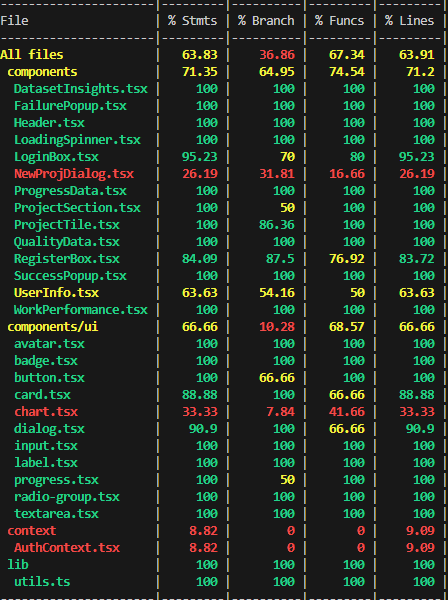
\includegraphics[width=0.5\linewidth]{FE_coverage.png}
    \caption{Front-end Unit Testing Coverage Results}
    \label{fig:FE_coverage}
\end{figure}

\bibliographystyle{plainnat}
\bibliography{../../refs/References}

\newpage{}
\section*{Appendix --- Reflection}

The information in this section will be used to evaluate the team members on the
graduate attribute of Reflection.

The purpose of reflection questions is to give you a chance to assess your own
learning and that of your group as a whole, and to find ways to improve in the
future. Reflection is an important part of the learning process.  Reflection is
also an essential component of a successful software development process.  

Reflections are most interesting and useful when they're honest, even if the
stories they tell are imperfect. You will be marked based on your depth of
thought and analysis, and not based on the content of the reflections
themselves. Thus, for full marks we encourage you to answer openly and honestly
and to avoid simply writing ``what you think the evaluator wants to hear.''

Please answer the following questions.  Some questions can be answered on the
team level, but where appropriate, each team member should write their own
response:


\begin{enumerate}
  \item What went well while writing this deliverable? 
  \item What pain points did you experience during this deliverable, and how
    did you resolve them?
  \item Which parts of this document stemmed from speaking to your client(s) or
  a proxy (e.g. your peers)? Which ones were not, and why?
  \item In what ways was the Verification and Validation (VnV) Plan different
  from the activities that were actually conducted for VnV?  If there were
  differences, what changes required the modification in the plan?  Why did
  these changes occur?  Would you be able to anticipate these changes in future
  projects?  If there weren't any differences, how was your team able to clearly
  predict a feasible amount of effort and the right tasks needed to build the
  evidence that demonstrates the required quality?  (It is expected that most
  teams will have had to deviate from their original VnV Plan.)
\end{enumerate}

\end{document}
